\documentclass{beamer}

\usepackage[T1,T2A]{fontenc}
\usepackage[utf8]{inputenc}

\usepackage{amsmath}
\usepackage{wrapfig}

\usepackage{bsuslides}

\graphicspath{ {img/} }

\title{ПРИМЕНЕНИЕ НЕЙРОННЫХ СЕТЕЙ В ЗАДАЧАХ АНАЛИЗА АУДИОДАННЫХ}
\subtitle{Курсовой проект}
\author{Ларин Егор Сергеевич}
\institute[БГУ]{Белорусский государственный университет \\ ФПМИ, КТС, 3 курс \\ руководитель: старший преподаватель Шолтанюк С. В.}
\date{Минск, 2022}

%\nofiles
\begin{document}

\frame{\titlepage}

\begin{frame}
	\frametitle{Введение}
	\begin{itemize}
		\item Распространение музыки и стриминговых сервисов делает актуальным разработку новых рекомендательных алгоритмов. 
		\item С задачей классификации музыки отлично справляются нейронные сети.
		\item В связи с этим предлагалось разработать проект, демонстрирующий существующие подходы анализа аудиоданных.
		\item Для тестирования созданных решений было необходимо создать набор данных из современной музыки.
	\end{itemize}
\end{frame}

\begin{frame}
	\frametitle{Признаки аудиоданных}
	\begin{enumerate}
		\item Преобразование Фурье.
		\item Мел-кепстральные коэффициенты (MFCC).
		\item Спектральные показатели контрастности.
		\item Хроматограмма по оконному преобразованию Фурье.
	\end{enumerate}
\end{frame}

\begin{frame}
	\frametitle{Применение мел-спектрограмм}
	\centering
	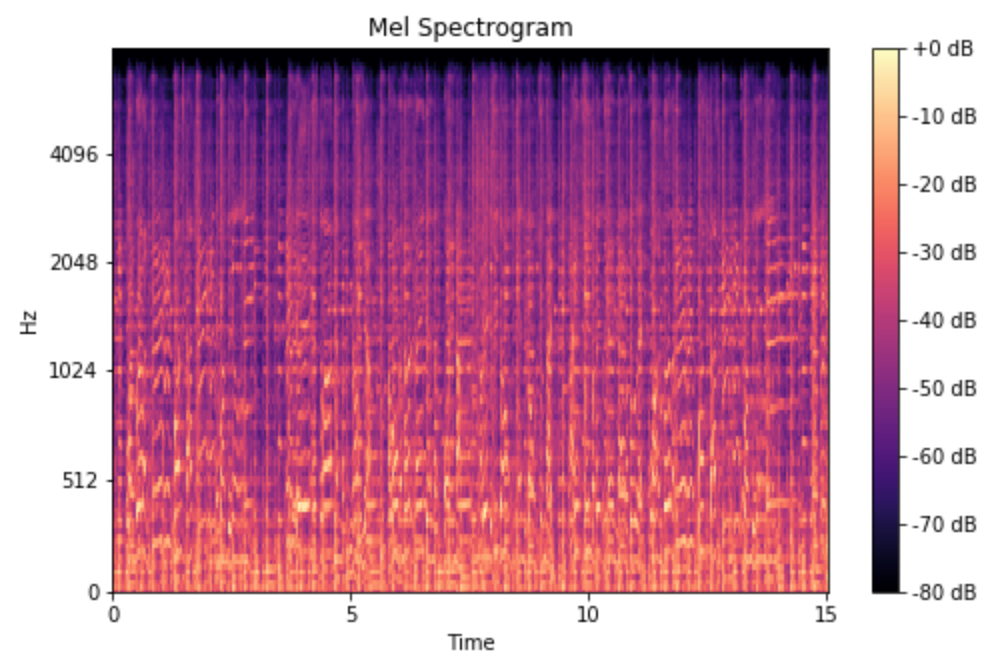
\includegraphics[height=7cm]{mel1.png}
\end{frame}

\begin{frame}
	\frametitle{Нейронная сеть}
	\begin{enumerate}
		\item 2 скрытых слоя на 128 нейронов и на 4 нейрона соответственно.
		\item Оптимизатор Adam.
		\item На основе Keras Tensorflow.
	\end{enumerate}
	\centering
	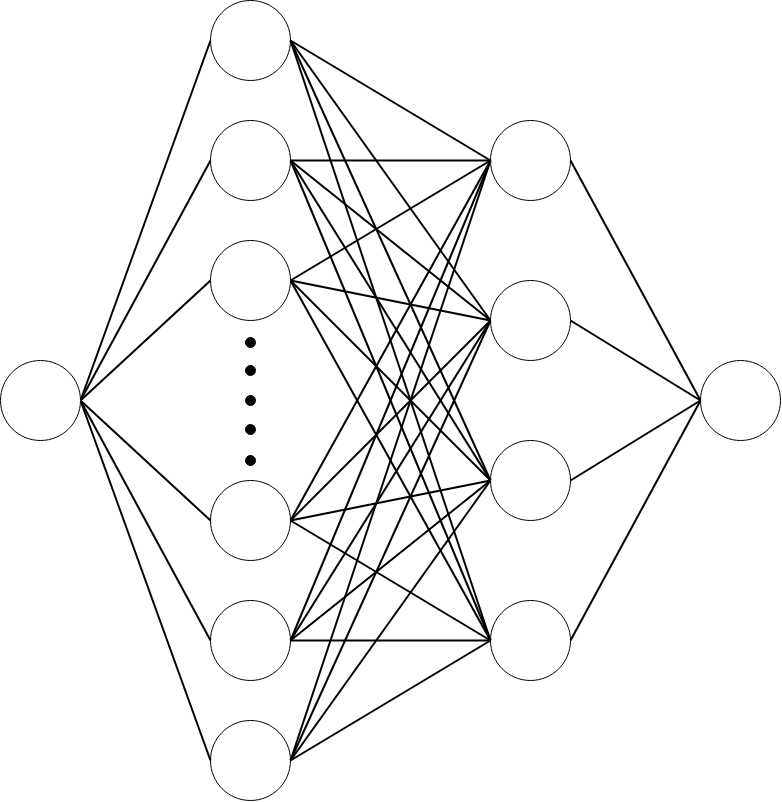
\includegraphics[height=5cm]{nn.png}
\end{frame}

\begin{frame}
	\frametitle{Кластеризация}
	\begin{enumerate}
		\item Случайный выбор центров кластеров.
		\item На основе scikit-learn.
	\end{enumerate}
	\centering
	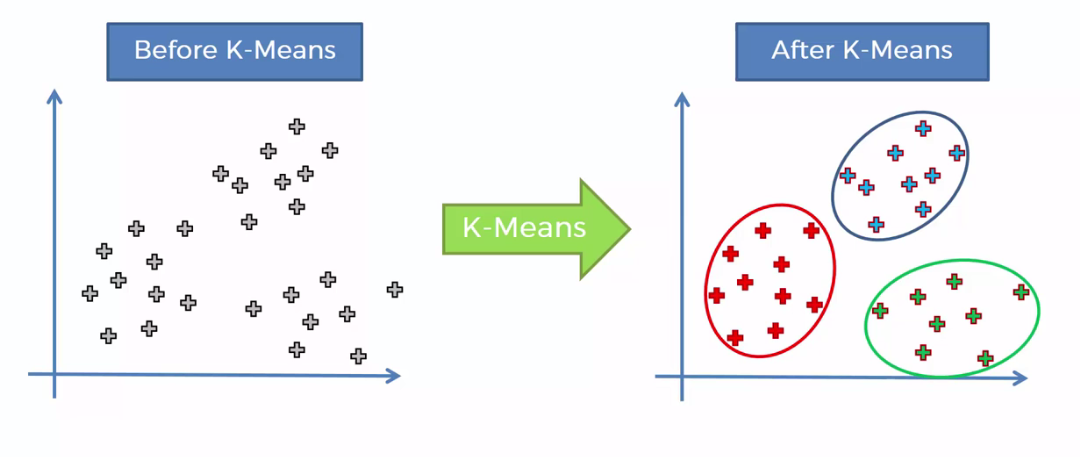
\includegraphics[height=5cm]{kmeans.png}
\end{frame}

\begin{frame}
	\frametitle{Результаты}
	\begin{itemize}
		\item k-means показывает 43\% точность.
		\item Нейронная сеть показала 78\% точность.
	\end{itemize}
	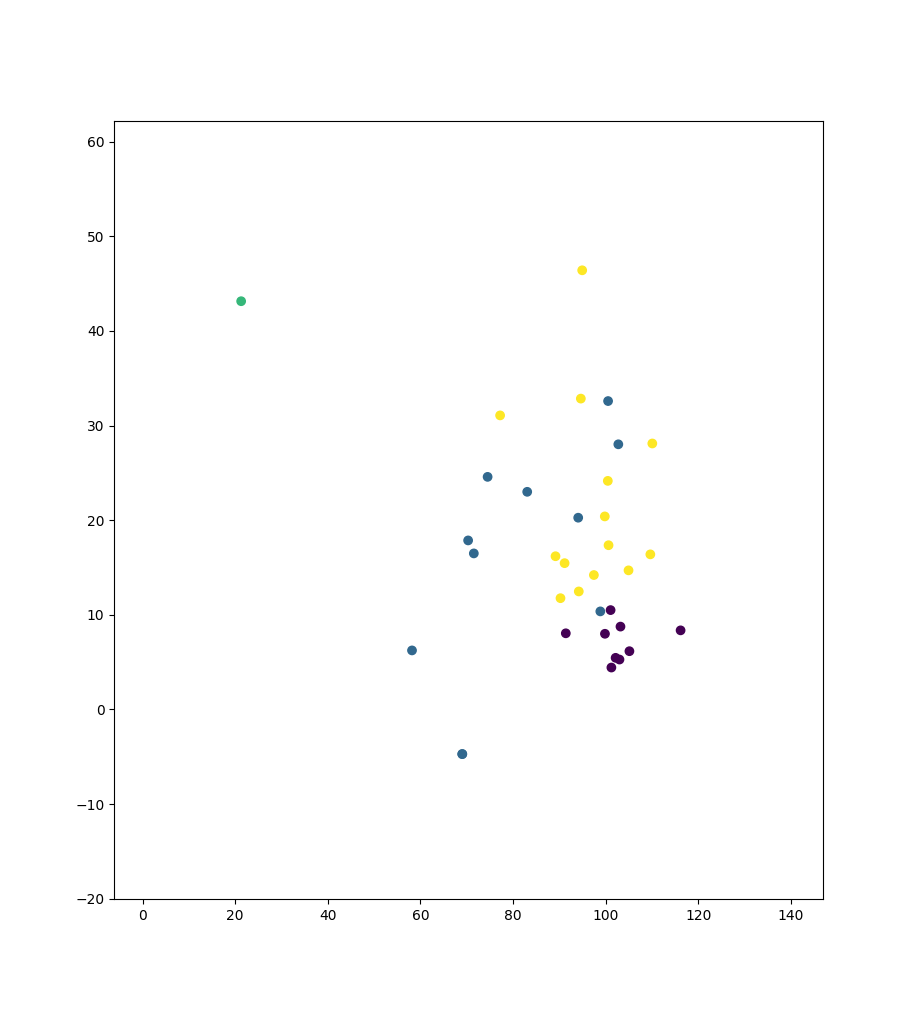
\includegraphics[width=0.475\textwidth]{Figure_1.png}
	\hfill
	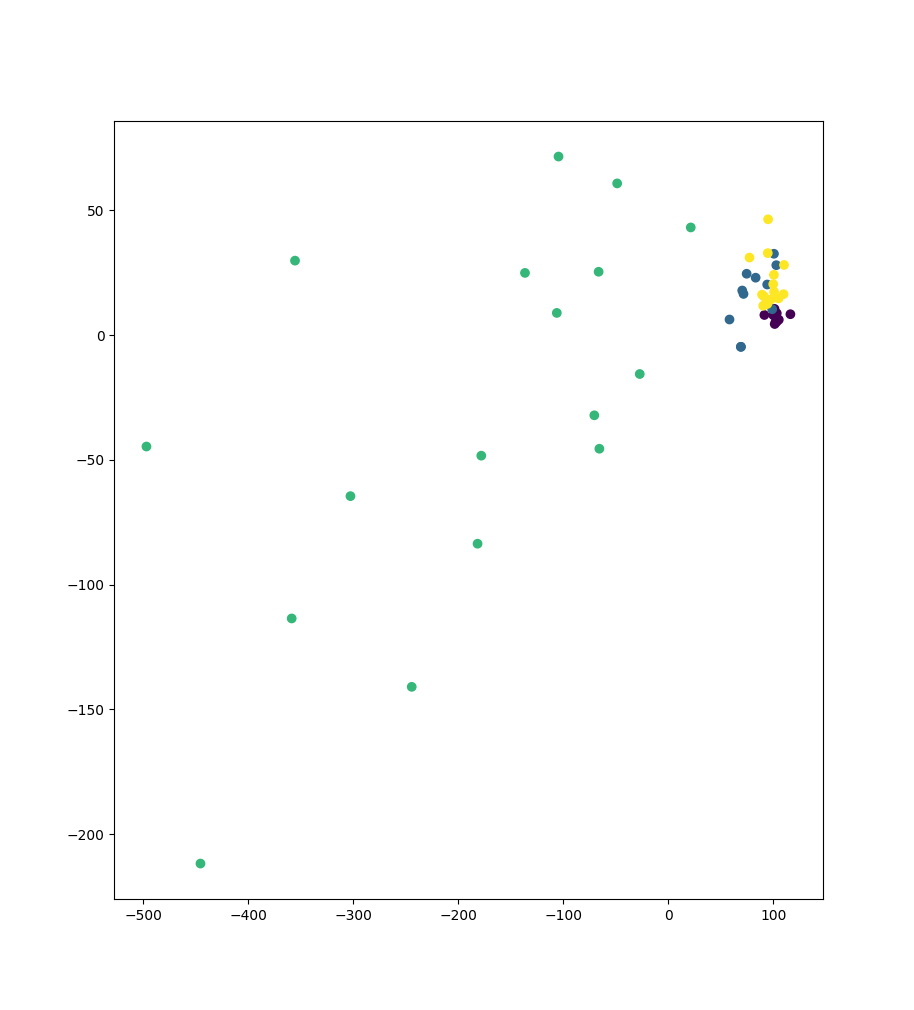
\includegraphics[width=0.475\textwidth]{Figure_2.png}
\end{frame}

\begin{frame}
	\frametitle{CNN}
	\centering
	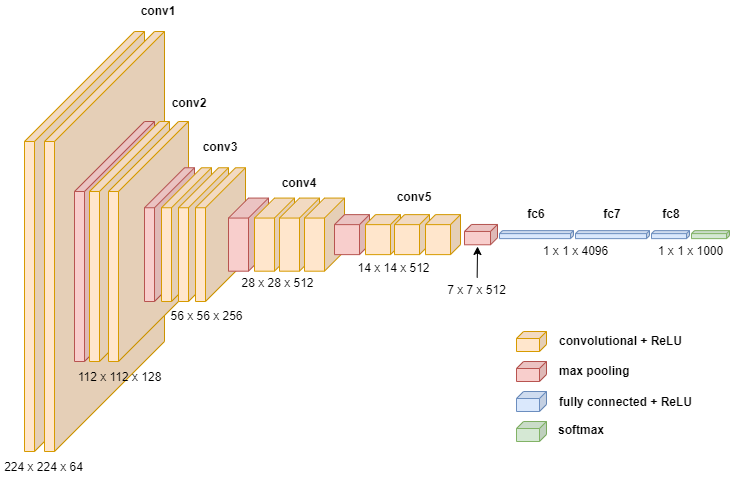
\includegraphics[height=7cm]{conv.png}
\end{frame}

\begin{frame}
	\frametitle{Заключение}
	\begin{itemize}
		\item Были разработаны два решения, демонстрирующие различные подходы к обучению.
		\item Создан собственный набор данных.
		\item Изучены исследования, которые могут стать основой для совершенствования построенных моделей.
	\end{itemize}
\end{frame}

\begin{frame}
	\frametitle{Источники}
	\begin{enumerate}
		\item Головко, В. А. Нейросетевые технологии обработки данных: учеб. пособие / В. А. Головко, В. В. Краснопрошин. – Минск : БГУ, 2017. – 263 с. – (Классическое университетское издание). – Режим доступа: http://elib.bsu.by/handle/123456789/193558. 
		\item Бредихин Арсентий Игоревич Алгоритмы обучения сверточных нейронных сетей // Вестник ЮГУ. 2019. №1 (52). Режим доступа: https://cyberleninka.ru/article/n/algoritmy-obucheniya-svertochnyh-neyronnyh-setey. 
		\item Choi J., Lee J., Park J., Nam J. Zero-shot Learning for Audio-based Music Classification and Tagging [Электронный ресурс] // arXiv.org. 2019. Режим доступа: https://arxiv.org/abs/1907.02670.
	\end{enumerate}
\end{frame}


\end{document} 
